\chapter{Exercise 06}
\extitle{Logistic Regression}
%%******************************************************************************%
%                                                                              %
%                                 Interlude                                    %
%                         for Machine Learning module                          %
%                                                                              %
%******************************************************************************%

\section*{Interlude - Evaluate}

\begin{figure}[h!]
  \centering
  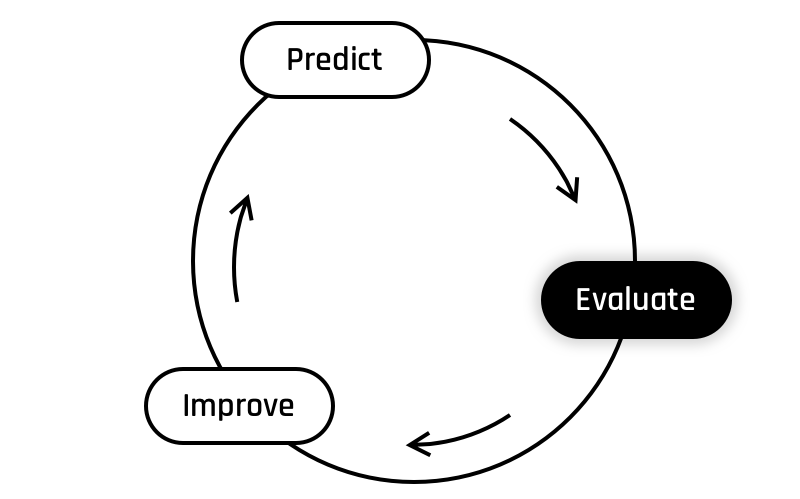
\includegraphics[scale=0.25]{assets/Evaluate.png}
  % \caption{cycle evaluate}
\end{figure}

\subsection*{Introducing the loss function}

How good is our model?  
It is hard to say just by simply looking at the plots!
We can clearly observe that certain regression lines seem to fit the data better than others, but it would be convenient to find a way to measure it. 

\begin{figure}[h!]
  \centering
  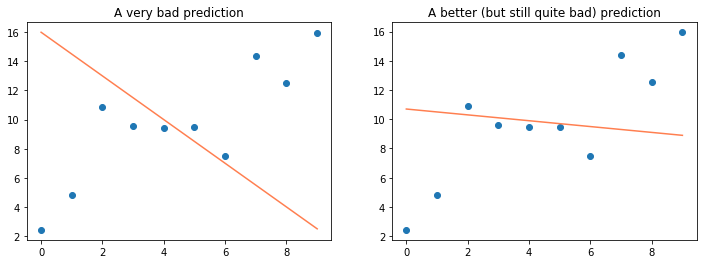
\includegraphics[scale=0.55]{assets/bad_prediction.png}
  \caption{bad prediction}
\end{figure}

To evaluate our model, we are going to use a \textbf{metric} called \textbf{the loss function} (sometimes called \textbf{cost function}).\\
\newline
The loss function tells us how bad our model is performing, how much it \textit{costs} us to use it, how much information we \textit{lose} when we use it.
If the model is good, we won't lose that much; if it's terrible instead, we will have a high loss!

The metric you choose will deeply impact the evaluation (and therefore also the training) of your model.

A frequent way to evaluate the performance of a regression model is to measure the distance between each predicted value ($\hat{y}^{(i)}$) and the real value it tries to predict (${y}^{(i)}$). The distances are then squared, and averaged to get one single metric, denoted $J$:

$$
J(\theta) = \frac{1}{2m}\sum_{i=1}^{m}(\hat{y}^{(i)} - y^{(i)})^2
$$

The smaller, the better! 

\begin{figure}[h!]
  \centering
  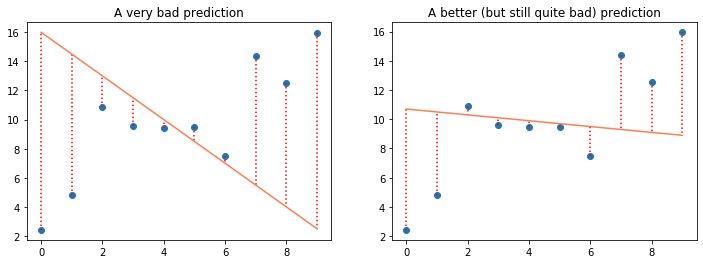
\includegraphics[scale=0.55]{assets/bad_pred_with_distance.png}
  \caption{bad prediction with distance}
\end{figure}

%\newpage
\turnindir{ex06}
\exnumber{06}
\exfiles{my\_logistic\_regression.py}
\exforbidden{sklearn}
\makeheaderfilesforbidden

% ================================= %
\section*{Objective}
% --------------------------------- %
The time to use everything you built so far has (finally) come!\\
\\
Demonstrate your knowledge by implementing a logistic regression classifier using 
the gradient descent algorithm.\\
\\
You must have seen the power of \texttt{numpy} for vectorized operations.
 Well let's make something more concrete with that.\\
\\
You may have taken a look at Scikit-Learn's implementation of logistic regression 
and noticed that the \textbf{sklearn.linear\_model.LogisticRegression} class 
offers a lot of options.\\
\\
The goal of this exercise is to make a simplified but nonetheless useful and powerful
 version, with fewer options.\\
\newpage
% ================================= %
\section*{Instructions}
% --------------------------------- %
In the \texttt{my\_logistic\_regression.py} file, write a \texttt{MyLogisticRegression} 
class as in the instructions given below:\\

\begin{minted}[bgcolor=darcula-back,formatcom=\color{lightgrey},fontsize=\scriptsize]{python}
class MyLogisticRegression():
	"""
	Description:
		My personnal logistic regression to classify things.
	"""
    def __init__(self, theta, alpha=0.001, max_iter=1000):
        self.alpha = alpha
        self.max_iter = max_iter
        self.theta = theta
        ... Your code here ...

	... other methods ...
\end{minted}
\\
You will add at least the following methods:
\begin{itemize}
  \item \texttt{predict\_(self, x)}
  \item \texttt{loss\_elem\_(self, y, yhat)}
  \item \texttt{loss\_(self, y, yhat)}
  \item \texttt{fit\_(self, x, y)}
\end{itemize}
\hint{You have already written these functions, you will just need a 
few adjustments in order for them to work well within your \textbf{MyLogisticRegression} class.}

% ================================= %
\subsection*{Examples}
% --------------------------------- %

\begin{minted}[bgcolor=darcula-back,formatcom=\color{lightgrey},fontsize=\scriptsize]{python}
import numpy as np
from my_logistic_regression import MyLogisticRegression as MyLR
X = np.array([[1., 1., 2., 3.], [5., 8., 13., 21.], [3., 5., 9., 14.]])
Y = np.array([[1], [0], [1]])
thetas = np.array([[2], [0.5], [7.1], [-4.3], [2.09]])
mylr = MyLR(thetas)

# Example 0:
mylr.predict_(X)
# Output:
array([[0.99930437],
       [1.        ],
       [1.        ]])

# Example 1:
mylr.loss_(X,Y)
# Output:
11.513157421577002

# Example 2:
mylr.fit_(X, Y)
mylr.theta
# Output:
array([[ 2.11826435]
       [ 0.10154334]
       [ 6.43942899]
       [-5.10817488]
       [ 0.6212541 ]])

# Example 3:
mylr.predict_(X)
# Output:
array([[0.57606717]
       [0.68599807]
       [0.06562156]])

# Example 4:
mylr.loss_(X,Y)
# Output:
1.4779126923052268
\end{minted}